\documentclass[sigconf]{acmart}
% Cleaning
\pagestyle{fancy} % removes running headers
\settopmatter{printacmref=false} % Removes citation information below abstract
\renewcommand\footnotetextcopyrightpermission[1]{} % removes footnote with conference information in first column
\pagestyle{plain} % removes running headers
\fancyhead{}
\settopmatter{printacmref=false, printfolios=false}
% Copyright
\setcopyright{none}
% \setcopyright{acmcopyright}
% \setcopyright{acmlicensed}
% \setcopyright{rightsretained}
% \setcopyright{usgov}
% \setcopyright{usgovmixed}
% \setcopyright{cagov}
% \setcopyright{cagovmixed}
\settopmatter{printacmref=false} % Removes citation information below abstract
\acmDOI{}

\usepackage{booktabs} % For formal tables
\usepackage{url}
\usepackage{algorithm}
\usepackage[noend]{algpseudocode}
\algtext*{EndWhile}% Remove "end while" text
\algtext*{EndIf}% Remove "end if" text
%\usepackage{flexisym}

\setlength{\parskip}{0pt}
\setlength{\parsep}{0pt}
\setlength{\headsep}{0pt}
\setlength{\topskip}{0pt}
\setlength{\topmargin}{0pt}
\setlength{\topsep}{0pt}
\setlength{\partopsep}{0pt}
%\linespread{0.95}
\usepackage{mdwlist}
\usepackage{amsmath}

\begin{document}
\title{nSense: Limits of Bias}
\author{Harrison Dean}
\affiliation{
  \institution{University of Victoria}
}
\email{harrisondean@uvic.ca}

\author{Carson Irvine}
\affiliation{
  \institution{University of Victoria}
}
\email{carsonirvine@uvic.ca}

\author{Xavier Roepcke}
\affiliation{
  \institution{University of Victoria}
}
\email{xavierroepcke@uvic.ca}

\author{Matthew Dunfee}
\affiliation{
 \institution{University of Victoria}
}\email{m1dunfee@uvic.ca}

\begin{abstract}
Bias tests for embeddings, such as WEAT, rely on hand-picked word lists. These word lists must separate words whose social group is part of their meaning (e.g., \textit{queen} for female) from words tied to a group only by stereotype (e.g., \textit{nurse} for female). To automate this separation, we propose nSense, a model that classifies words in sentences as \textit{innate}, \textit{derived}, or \textit{neutral}. nSense uses the word's contextual BERT embedding and a random forest trained on StereoSet, and is evaluated on words it has never seen. The code base, along with instructions, can be found at:

\noindent https://github.com/Hammerhead-lab/nSense.
\end{abstract}

\keywords{Embedding bias, AI, vector space, innate bias, derived bias}
\maketitle


\section{Problem Definition}
Our goal is to identify, for a word in a sentence about a social group, whether the group is part of the word's meaning, the word is tied to the group by stereotype alone, or neither. Bias tests for embeddings depend on word lists that make this distinction, yet prior work either leaves stereotyped and neutral words mixed or labels them by hand \cite{bolukbasi2016man}. Here, we provide a formal statement of the problem after which we propose our approach in detail in the next section.

We view this problem as an instance of multi-class classification. Let $\mathbb{G}$ be a set of social groups on three axes: gender, race/nationality, and religion. An observation $o = (s,i)\in \mathbb{O}$ pairs a sentence $s$ about a target group $g\in \mathbb{G}$ with a character span $i$ that selects a word $w$ in $s$. The class $y(o)\in \mathbb{Y}$ is defined relative to $g$:
\begin{equation}\label{label}
y(o)= \begin{cases}
    \text{innate} & \text{if } g \text{ is part of the meaning of } w,\\
    \text{derived} & \text{if } w \text{ is tied to } g \text{ only by stereotype,}\\
    \text{neutral} & \text{otherwise}
\end{cases}
\end{equation}
The goal of bias detection is to learn $f: \mathbb{O} \rightarrow \mathbb{Y}$ such that $f(o) = y(o)$, including for words not seen in training.

\section{Proposed Approach}\label{approach}
Our proposed bias detection method seeks to classify word spans as innate, derived, or neutral using labels constructed from StereoSet\cite{nadeem2020stereoset}. Each sentence is passed through pretrained BERT to produce a 768-dimensional vector representation of the selected word span. A random forest with 500 decision trees then learns to predict the word span's class from this vector. The classifier is evaluated using five-fold grouped cross-validation, keeping the training and testing word groups separate, and then its performance is compared with four baselines using macro-F1. 

\subsection{Observations (StereoSet)}
We construct observations from StereoSet's intrasentence validation data containing single-sentence examples focusing on gender, race/nationality, and religion. Each StereoSet item contains a target group term and sentence variants labeled either stereotype, anti-stereotype, or unrelated. An observation o consists of a sentence s and a selected word span i represented as o = (s, i), with each observation being paired with a reference label. We assign innate to the target term in the stereotype sentence, derived to the word filling its blank, and neutral to the fill word in the unrelated sentence. We excluded anti-stereotype sentences and profession items from our observations, as they do not fit the three classes. As well, we set aside derived or neutral spans that match a retained group term. This process resulted in 3,857 labeled observations, which are the input for the next stage, BERT encoding.

\subsection{Encoding (BERT)}
To establish credibility, the model, like the dataset, was chosen to mirror the research in the topic literature. BERT-base was among the models evaluated in the original StereoSet paper \cite{nadeem2020stereoset}, and bert-base-uncased is the BERT model used in bias-bench \cite{meade-etal-2022-empirical}. The reason uncased is used here is because the boundaries include innate words, which include proper nouns, and we want to exclude case-sensitive details from the vectors to avoid the random forest learning to treat those groups differently on that feature alone. BERT configuration includes being frozen with no fine-tuning, using the final hidden layer, mean pooling over subword pieces, and one 768-dimensional vector per target word in its encoded sentence. These vectors are the forest’s input.

\subsection{Random Forest Classifier}
Given the 768-dimensional vector representation $x_o \in \mathbb{R}^{768}$ extracted for each labeled word, we train a random forest model~\cite{breiman2001random} $c: \mathbb{R}^{768} \rightarrow \{\textit{innate}, \textit{derived}, \textit{neutral}\}$ to classify each word. A random forest works by building an ensemble of decision trees. In our setup, $T = 500$ individual trees---where each tree is trained on a random bootstrap sample of the rows in the training set. At every decision point (or split) in a tree, the algorithm randomly picks a small subset of features (here, $\lfloor\sqrt{768}\rfloor = 27$ dimensions) and selects the threshold that best splits the data into distinct classes. The tree keeps splitting the data into narrower branches until every final leaf node contains only a single class.

When making a prediction for a word vector $\mathbf{x}_o$, each tree calculates a probability distribution across the three classes, and the forest averages these probabilities together:
$$c(x_o) = \arg\max_{y} \frac{1}{T} \sum_{t=1}^{T} p_t(y \mid x_o)$$
The final predicted label is simply the class with the highest average probability $p_t$ across all 500 trees. Aside from setting $T = 500$ and locking the random seed to 503, we rely on the standard scikit-learn default settings~\cite{pedregosa2011scikit}. We deliberately skip hyperparameter tuning because generic random forests consistently deliver strong performances~\cite{probst2019hyperparameters}.

To evaluate how well our model generalizes to unseen words, we run 5-fold cross-validation using GroupKFold~\cite{roberts2017cross}. We group the rows by their base word (using the word's lemma, or the normalized target word for innate entries). This strict grouping ensures that no single word ever appears in both the training set and the test set within the same fold, preventing the model from simply memorizing specific words.

We measure performance using macro-averaged F1
score~\cite{sokolova2009systematic}, which treats all three target
classes equally regardless of how many examples each class has. We report the mean and standard deviation of the macro-F1 score across all five test folds. In addition, we measure feature importance by running permutation importance on each held-out test fold~\cite{breiman2001random, fisher2019all}. To judge our model's performance fairly, we evaluate four baseline models: a single cosine direction tree, a part-of-speech tag classifier, a word frequency classifier, and a context-only forest. We then use the exact same cross-validation folds and scoring metrics.


\begin{algorithm}[t]
\caption{Classifying words as innate, derived, or neutral}
\label{alg:nsense}
\small
\begin{algorithmic}[1]
\Statex \textbf{Inputs:}
\Statex \hspace{1em} $\mathcal{I}$, StereoSet items, each with a target word $\tau$,
\Statex \hspace{2em} a stereotype sentence $s^{+}$, and an unrelated sentence $s^{-}$;
\Statex \hspace{1em} $\mathcal{B}$, pretrained BERT encoder;
\Statex \hspace{1em} $K$, number of cross-validation folds;
\Statex \textbf{Output:}
\Statex \hspace{1em} $c^{*}$, trained random forest;
\Statex \hspace{1em} $\overline{F1}$, mean macro-F1 over held-out folds;
\Statex \textbf{Initialization:}
\Statex \hspace{1em} $\mathcal{R}=\emptyset$, set of labeled words;
\Statex \hspace{1em} set\_seed($\sigma$);
\Statex \rule{\linewidth}{0.4pt}

\Procedure{nSense}{$\mathcal{I},\mathcal{B},K,\sigma$}
  \ForAll{items $(\tau,s^{+},s^{-})\in\mathcal{I}$}
    \State $w^{+}\gets$ fill word of $s^{+}$
    \State $w^{-}\gets$ fill word of $s^{-}$
    \State $\mathcal{R}\gets\mathcal{R}\cup\{(s^{+},\tau,\textit{innate}),\;
           (s^{+},w^{+},\textit{derived}),\;(s^{-},w^{-},\textit{neutral})\}$
  \EndFor
  \Statex
  \ForAll{$(s,w,y)\in\mathcal{R}$}
    \State $\mathbf{x}\gets$ mean of $\mathcal{B}(s)$ token vectors of $w$
  \EndFor
  \Statex
  \State split $\mathcal{R}$ into $K$ folds so that each word group is in one fold only
  \For{each fold $k$}
    \State train random forest on the other folds; predict fold $k$
    \State $F1_k\gets$ macro-F1 on fold $k$
  \EndFor
  \Statex
  \State $c^{*}\gets$ random forest trained on all of $\mathcal{R}$
  \State \Return $c^{*}$, $\overline{F1}=\operatorname{mean}_k F1_k$
\EndProcedure
\end{algorithmic}
\end{algorithm}

\begin{figure}[t]
\centering
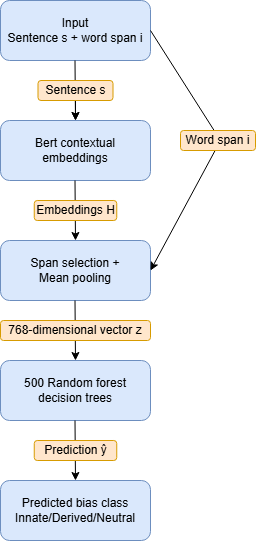
\includegraphics[width=0.4\columnwidth]{Images/nSense_Figure.png}
\caption{The nSense classification pipeline.\label{nSense_Pipeline}}
\end{figure}



\bibliographystyle{ACM-Reference-Format}
\bibliography{bibliography.bib}

\end{document}
